\documentclass{article}
\usepackage[utf8]{inputenc}
\usepackage{graphicx}
\usepackage{blindtext}
\usepackage{subfiles}
\usepackage[colorlinks = false]{hyperref}
\usepackage[table]{xcolor}
\usepackage{rotating}
\usepackage{adjustbox}


\usepackage[TS1,T1]{fontenc}

\usepackage[normalem]{ulem}
\usepackage{fancyhdr}
\pagestyle{fancy}
\fancyhf{}
\rhead{Measuring Rhetorical Similarity - Appendix}
\lhead{Nicolai Berk}
\cfoot{\thepage}

\useunder{\uline}{\ul}{}


\title{ONLINE APPENDIX\newline Measuring Rhetorical Similarity with Supervised Machine Learning}
\author{Nicolai Berk}
\date{\today}


\begin{document}


\subsection*{Appendix A}

\begin{table}[ht!]
\noindent\adjustbox{max width=\textwidth}{%
\begin{tabular}{|l|l|l|l|l|l|l|}
\hline
\textbf{Classifier}   & \textbf{Vectorizer} & \textbf{Stemmed} & \textbf{F1}   & \textbf{Accuracy} & \textbf{Precision} & \textbf{Recall} \\ \hline
Logistic   Regression & tfidf               & raw              & \textbf{0.59} & 0.87              & 0.55               & 0.64            \\ \hline
SVM                   & tfidf               & raw              & \textbf{0.57} & 0.88              & 0.59               & 0.56            \\ \hline
Logistic   Regression & tfidf               & stemmed          & \textbf{0.55} & 0.83              & 0.45               & 0.7             \\ \hline
Multinomial NB        & tfidf               & raw              & \textbf{0.55} & 0.85              & 0.48               & 0.64            \\ \hline
Multinomial NB        & tfidf               & stemmed          & \textbf{0.54} & 0.84              & 0.47               & 0.64            \\ \hline
SVM                   & tfidf               & stemmed          & \textbf{0.54} & 0.84              & 0.47               & 0.62            \\ \hline
Logistic   Regression & count               & raw              & \textbf{0.49} & 0.84              & 0.46               & 0.53            \\ \hline
Logistic   Regression & count               & stemmed          & \textbf{0.48} & 0.83              & 0.43               & 0.55            \\ \hline
Multinomial NB        & count               & raw              & \textbf{0.46} & 0.85              & 0.48               & 0.45            \\ \hline
Multinomial NB        & count               & stemmed          & \textbf{0.46} & 0.85              & 0.47               & 0.45            \\ \hline
SVM                   & count               & raw              & \textbf{0.46} & 0.83              & 0.42               & 0.5             \\ \hline
SVM                   & count               & stemmed          & \textbf{0.45} & 0.81              & 0.4                & 0.52            \\ \hline
\end{tabular}
}
\caption{Performance of different qualifiers on German data, sorted by F1-score. $F_1 = 2*\frac{precision*recall}{precision+recall}$ }
\end{table}



\subsection*{Appendix B1}
\begin{figure}[ht!]
    \centering
    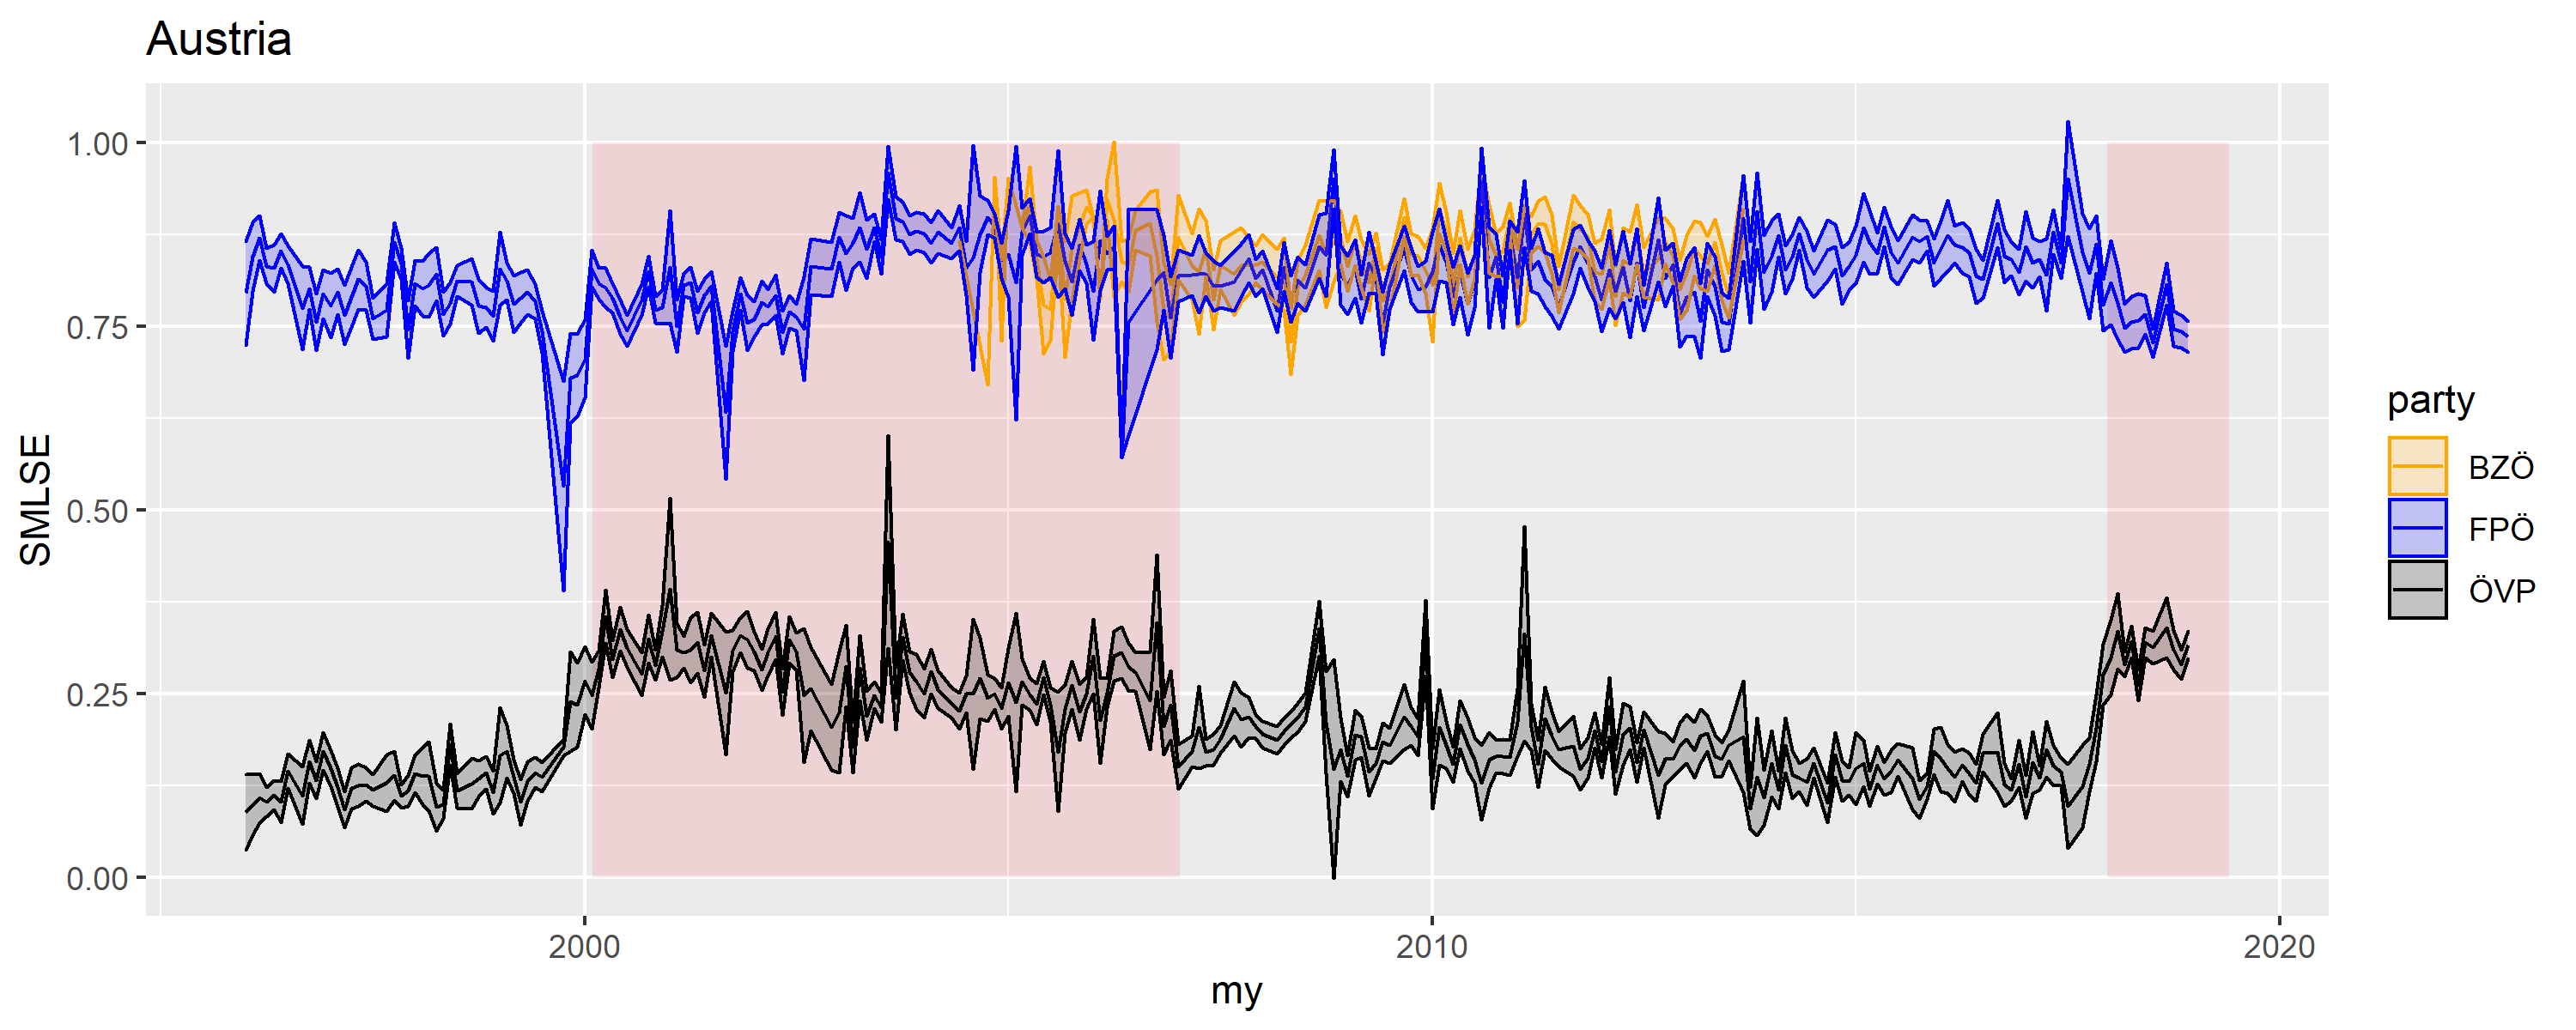
\includegraphics[width=\textwidth]{AT/vis/AT_fpvpbz_paper.png}
    \caption{Estimates for Austria including BZÖ}
    \label{fig:bzoe}
\end{figure}

\subsection*{Appendix B2}
\begin{figure}[ht!]
    \centering
    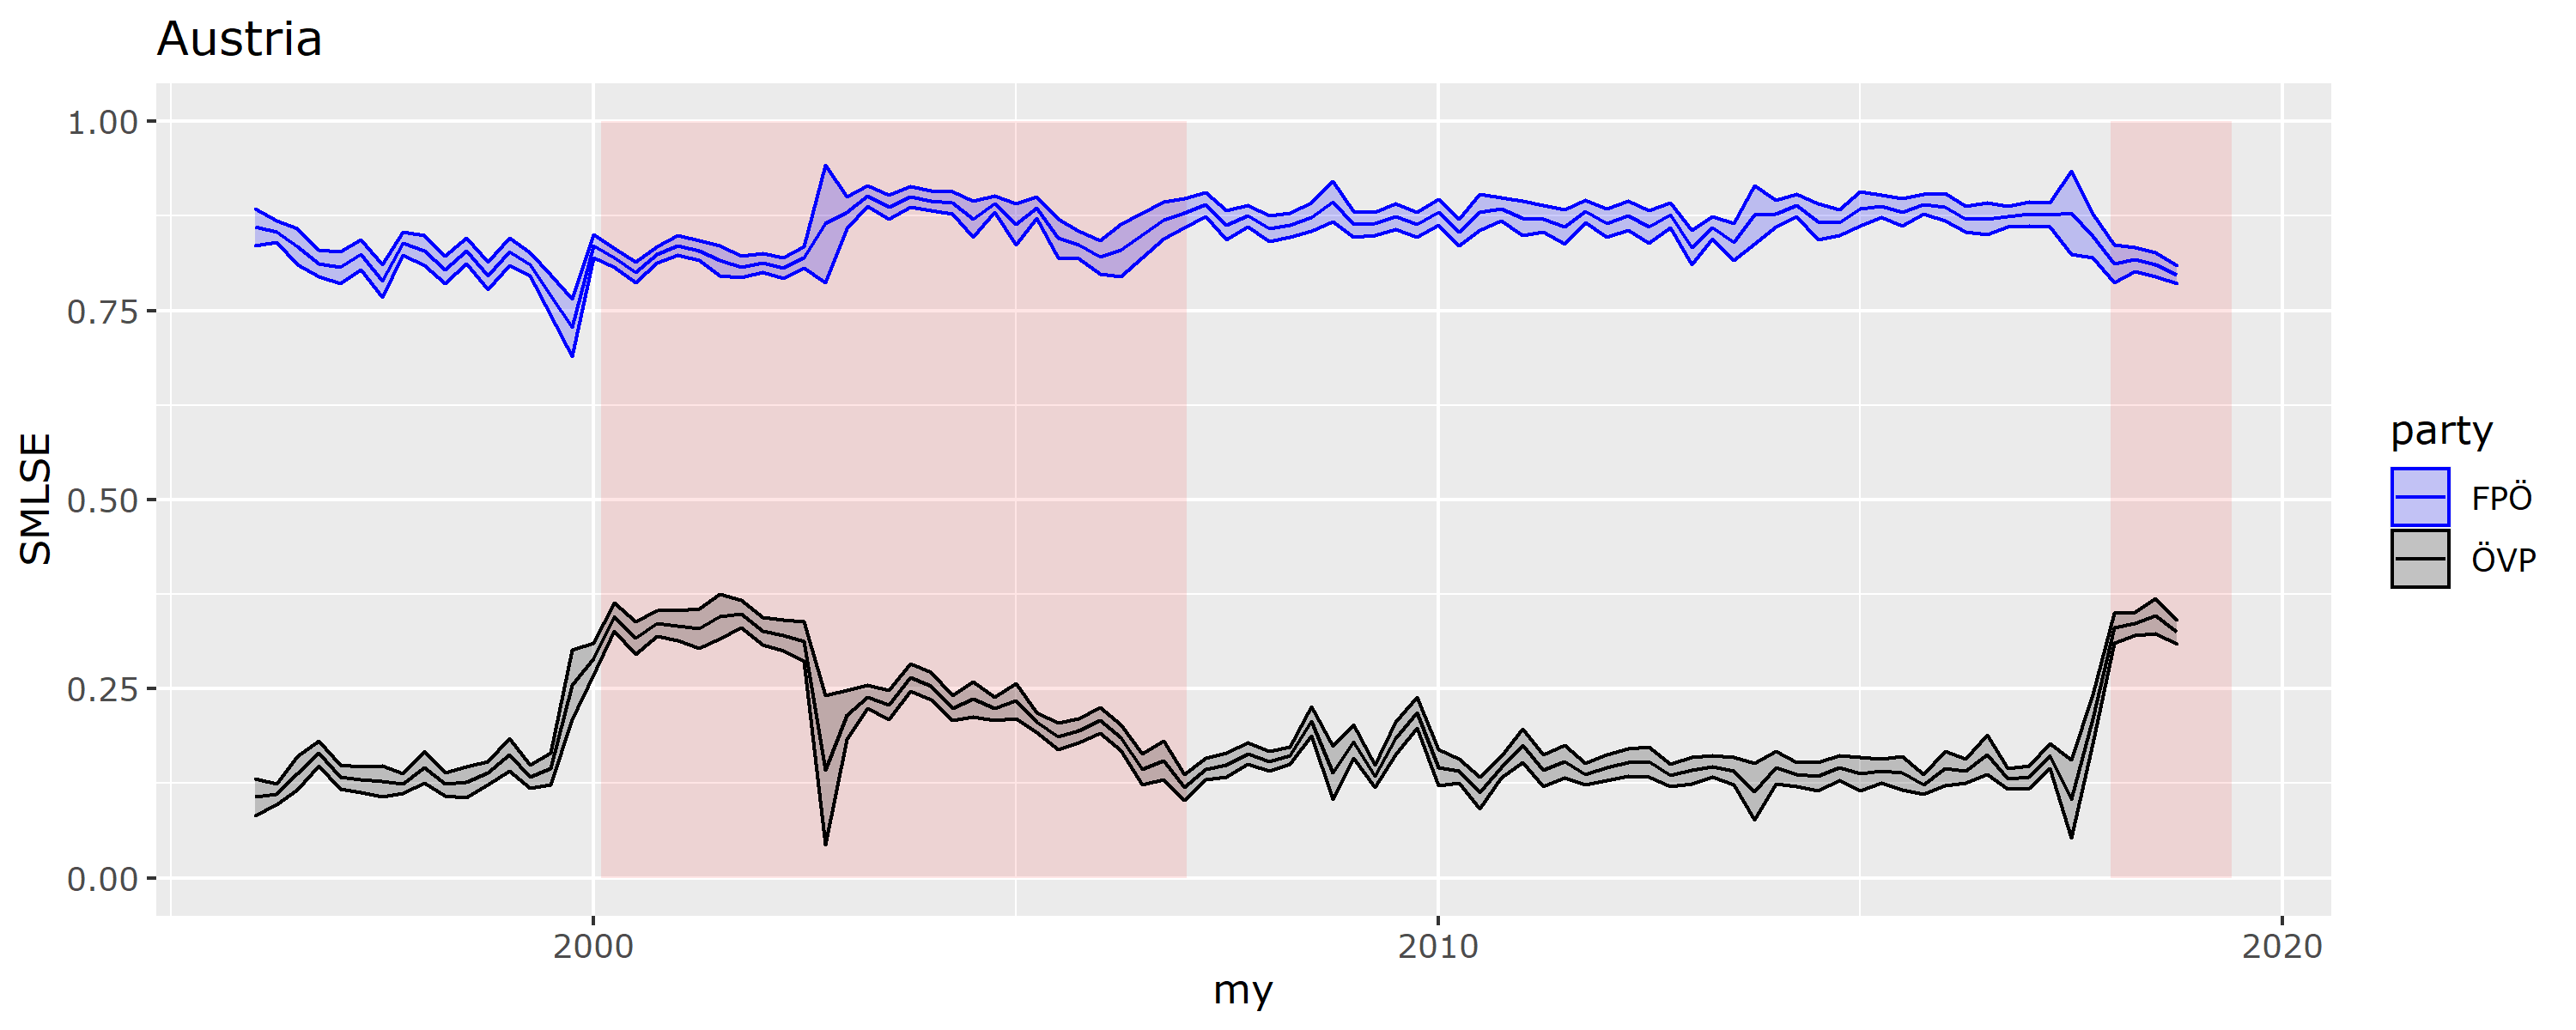
\includegraphics[width=\textwidth]{AT/vis/AT_fpvp_fpest_paper.png}
    \caption{Estimates for Austria trained to detect FPÖ-speeches only.}
    \label{fig:fponly}
\end{figure}


\subsection*{Appendix C}

% describe dutch gov formations

\begin{figure}[ht!]
    \centering
    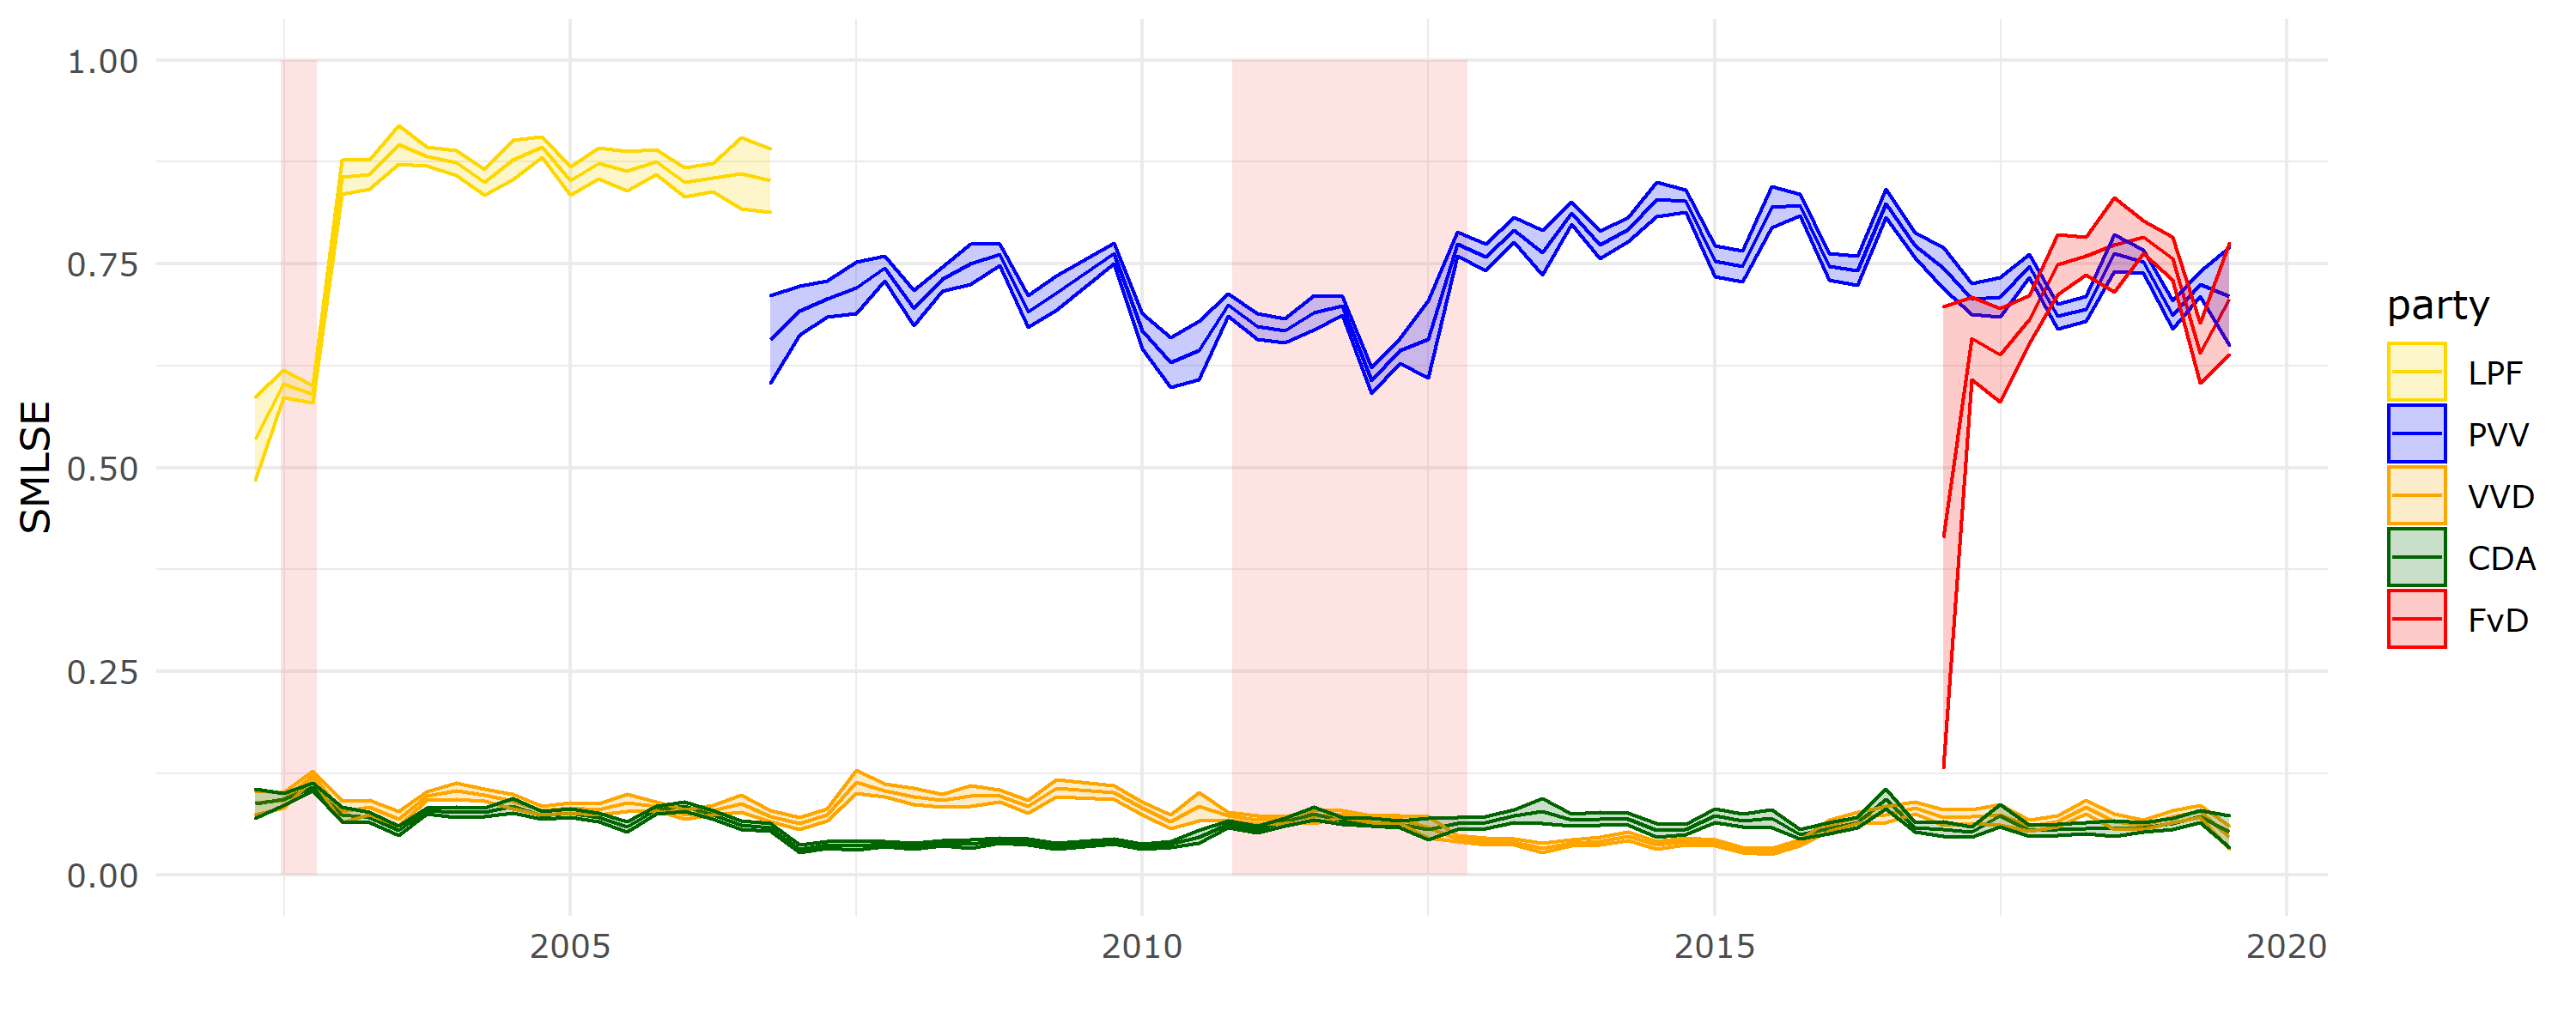
\includegraphics[width=\textwidth]{NL/vis/nl_vvd_cda_rr.png}
    \caption{Estimates for the Netherlands including CDA and FvD.}
    \label{fig:cda}
\end{figure}

The Netherlands saw only one formal coalition government between radical-right and centre-right, but an additional minority government supported by the radical-right PVV. In 2002 the \textit{Lijst Pim Fortuyn} (LPF) brought unprecedented volatility and polarisation into Dutch politics (\cite{Bischof2019a, VanderBrug2003}). Only formed about three months preceding the election, the party gained wide attraction due to its charismatic leader, a strong media presence and its distinctive anti-immigration stance (\cite{Koopmans2009}). On election day, nine days after the party leader Pim Fortuyn was assassinated, the party came in second with 17\% of the vote and formed a coalition with the christian-democrat CDA and the centre-right VVD. Having lost its founding father and as a result of its rapid success, the party was unprepared for government and was turmoiled by internal power struggles. This peaked when two LPF ministers stopped talking to each other. As a result, CDA and VVD broke the coalition only 87 days after its formation (\cite{Heinisch2003, Lucardie2007LPF}). I expect especially the LPF to become less distinctive here, as the party members decide to enter a coalition government. Similarly, CDA and VVD should become more alike the LPF in government.\par

The co-operation of VVD, CDA and PVV in 2010 did not result in a formal majority coalition (partly due to internal conflicts in the CDA regarding a coalition with the radical-right PVV), but a 'supported minority government'. This was the first minority government formed in the Netherlands since 1922. VVD and CDA staffed the cabinet, while the PVV only promised support on major issues. As this support was settled in a formal agreement, this government became basically a 'majority government in disguise' (\cite{Strom1990, VanHolsteyn2011}). In fact, the government cooperated very little with the opposition even compared to full majority governments - this is likely an outcome of the sorting of parties into a right-wing government and a left-wing opposition but underlines the similarity of this government to classic majority coalitions (\cite{Otjes2014}). As a result, I expect an increased similarity of the coalition partners, slightly less than in a majority coalition. \par

The lower row of figure \ref{fig:govs} shows the monthly average similarity estimate in the Netherlands for PVV, LPF, and VVD\footnote{CDA and FvD were excluded to maintain readability. The full plot can be found in figure \ref{fig:cda}, appendix C.}. The LPF is rather similar to all other parties when in government, obtaining a distinctiveness estimate of only around 60\%\footnote{This value can be interpreted as the confidence with which the classifier identifies LPF speeches as such.} throughout the time governing. Once the party leaves the government, the party becomes very distinctive again. For the VVD, we can observe a slightly increased score when governing with the LPF. For the supported minority government in 2010, things are far less clear. The VVD's estimate seems to remain rather stable, with possibly a slight \textit{decrease}, while the PVV becomes much less distinctive just \textit{before} signing the support agreement. Afterwards, the PVV stays somewhat indistinctive throughout the time supporting the government at around 60\% - 70\%. After the time in government, the party's communication becomes more distinctive again.\par

T-tests confirm these observations. The LPF does show a significantly decreased distinctiveness in government (t=-6.15, p$<$0.01), as does the PVV (t=-5.36, p$<$0.001). The VVD only shows slightly increased similarity to the respective radical-right party when governing with the LPF (t=3.21, p$<$0.1), but when supported by the PVV, this effect becomes virtually zero (t=0.6, p=0.55). The CDA is assigned similar SMLSEs, though more clearly reacting to the LPF (t=7.1, p$<$0.01), but neither to the PVV (t=0.96, p=0.34). Overall, the VVD is not significantly affected by governing with a radical-right party (t = 1.64, p$>$0.1), while the CDA is significantly changing its rhetoric (t=2.01, p$<$0.05).\par

Additionally, throughout the time in government, the LPF becomes less distinctive, while the VVD seems to become more similar. This is in line with an ideological shift in the VVD's manifesto, which took up a more anti-immigrant position (\cite{Pennings2003}), while the LPF dropped some of it's populist rhetoric (\cite{Lucardie2007LPF}). For the PVV, a shift towards the centre is visible before the formation of the minority support government - possibly signalling willingness to govern, similar to Haider's FPÖ preceding the Austrian elections in 2000.\par

\subsection*{Appendix D}

% plot changes in similarity FPOE and OEVP, surrounding takeover Kurz and election 201
%   (need to change visualisations from sim to party to sim OF party)

\subsection*{Appendix E}
\begin{table}[ht!]
\begin{tabular}{|l|l|l|l|}
\hline
Word        & Contribution & Word           & Contribution \\ \hline
minister    & 50.2         & mij            & 8.4          \\ \hline
kunnen      & 16.5         & kabinet        & 8.2          \\ \hline
vind        & 15.8         & hij            & 7.8          \\ \hline
Algerije    & 12           & ministerie     & 7.3          \\ \hline
ben         & 11.7         & Het            & 7.1          \\ \hline
motie       & 10.8         & Arabië         & 7.1          \\ \hline
LPF         & 10.7         & imam           & 7            \\ \hline
AIVD        & 9.9          & terroristische & 6.9          \\ \hline
Wij         & 9.9          & groot          & 6.9          \\ \hline
zeker       & 9.6          & Europa         & 6.8          \\ \hline
mening      & 9.6          & onderzoek      & 6.2          \\ \hline
Defensie    & 9.5          & Dutchbat       & 6.2          \\ \hline
terroristen & 9.4          & man            & 6            \\ \hline
Dat         & 9.3          & moskeeën       & 5.6          \\ \hline
Saoedi      & 8.6          & moskee         & 5.5          \\ \hline
\end{tabular}
\caption{Thirty words with the strongest positive contribution in Wilders' speeches as a member of the VVD 2004.}
\label{tab:wilders}
\end{table}




\end{document}